%!TeX spellcheck = en_US
\documentclass[12pt,a4paper,USenglish]{article}      % Specifies the document class
\usepackage[utf8]{inputenc}
\usepackage[T1]{fontenc,url}
\usepackage{babel,csquotes,newcent,textcomp}
\usepackage[backend=biber,sortcites]{biblatex}
\usepackage{graphicx}
%\usepackage{graphics}
%\usepackage{listings}

\usepackage{listings}
\usepackage{color}
\usepackage{comment}
\usepackage[nokeyprefix]{refstyle}

\definecolor{dkgreen}{rgb}{0,0.6,0}
\definecolor{gray}{rgb}{0.5,0.5,0.5}
\definecolor{mauve}{rgb}{0.58,0,0.82}

\lstset{frame=tb,
  language=Java,
  aboveskip=3mm,
  belowskip=3mm,
  showstringspaces=false,
  columns=flexible,
  basicstyle={\small\ttfamily},
  numbers=left,
  numberstyle=\tiny\color{gray},
  keywordstyle=\color{blue},
  commentstyle=\color{dkgreen},
  stringstyle=\color{mauve},
  breaklines=true,
  breakatwhitespace=true,
  tabsize=3
}

\graphicspath{ {./images/} }

%\addbibresource{References.bib}

\title{Methodology}  % Declares the document's title.

%\newcommand{\ip}[2]{(#1, #2)}

\begin{document}             % End of preamble and beginning of text.
%\maketitle                   % Produces the title.
\section{Simulation}
\subsection{Introduction}
The tests that was done in chapter three and four the DRAM and NVDIMM have been doing the same type of work. This chapter will be about DRAM and NVDIMM doing different types of work. 
There will be a group of threads calculating data on DRAM. While this is going on there will be another group of threads copying the latest set of calculated data to NVDIMM and analyzing the data on NVDIMM.
The purpose of this is to find out if NVDIMM can work on other tasks and understand how NVDIMM behave when working other threads are working on DRAM.
The chapter will start by testing the simulation using only DRAM in order to see what kind of performance is possible. Afterward another version of the program will be tested where both DRAM and NVDIMM is being used. 

\subsection{DRAM only}
\label{section:DramOnly}
\subsubsection{Description of code}
The code at start by taking a time measurement before the while-loop in line 4 in listings \ref{lst:DramOnlyMain} by on of the threads. This time measurement will be ended after the while-loop at line 41 by one thread. Since there is a barrier at line 38 the time measurement will only end when all the threads have left the while-loop.

The While-loop at line 6 will be repeated for 5000 times and there is a barrier in line 7 to ensure that all threads are finished with the previous iteration before starting a new iteration. One thread will start by entering a single in line 8 and do all the work only one thread can do such as increase n by one, zero out diff and average and a part of a formula that will be used in data generation.
The description of data generation will be done in section \ref{sec:dramOnlyDatagen}.

After the data generation all the threads will wait the barrier at line 19 before one thread enter the single at line 20. The thread will swap the arrays x and xk\_1 before starting a new time measurement at line 26.
The threads will move on to analyzing the data generated and this will be described at section \ref{sec:dramOnlyAnalyze}.

The threads will wait for all the threads to complete analyzing the data at line 31 before on thread enter a new single at line 32 where it will first start by calculating an average and after that it will end the time measurement that was started at line 26. This is the time measurement of the analyzing part of the code, the time it takes to analyze the data in all iteration will be add to one variable called analyze\_time. This is the end of the while-loop and the code will either return to line 7 or exit the while-loop

The time measurement of the data generation will be found by subtracting analyze\_time from the time measurement that was taken before and after the code. 

%[caption=while-loop]
\begin{lstlisting}[caption={DRAM only version of the simulation code.},escapeinside={{/*!}{!*/}}, label={lst:DramOnlyMain}]
double double_temp;
#pragma omp single
{
	data_generation_time, = mysecond();
}
while( n<5000 ){
	#pragma omp barrier
	#pragma omp single
	{
		n++;
		diff=0.0;
		average = 0;
		//completes the first part of the formula.
		Wk_1_product = (omd + (d*Wk_1))*iN;
	}
	
	Data generation, see section /*!\ref{sec:dramOnlyDatagen}!*/
	
	#pragma omp barrier
	#pragma omp single
	{
		temp_x = xk_1;
		xk_1 = x;
		x = temp_x;
		//starting time measurement of calculation.
		temp_calc=mysecond();
	}
	
	Analyzing the data, see section /*!\ref{sec:dramOnlyAnalyze}!*/
	
	#pragma omp barrier
	#pragma omp single
	{
		average *= iN;
		analyze_time+=mysecond()-temp_calc;
	}
}
#pragma omp barrier
#pragma omp single
{
	data_generation_time, = mysecond() - data_generation_time;
}
\end{lstlisting}
The code shown in listing \ref{lst:DramOnlyTimeMeasurement} is the function used to take the time measurement. This function have been copied from the Stream benchmark code. 
\begin{lstlisting}[caption={Function that that is used for measure time},escapeinside={{/*!}{!*/}}, label={lst:DramOnlyTimeMeasurement}]
double mysecond(){
	struct timeval tp;
	struct timezone tzp;
	int i;
	i = gettimeofday(&tp,&tzp);
	return ( (double) tp.tv_sec + (double) tp.tv_usec * 1.e-6 );
}
\end{lstlisting}
%\clearpage
\subsubsection{Data generation}
\label{sec:dramOnlyDatagen}
\begin{comment}
The arrays x and xk\_1 are double arrays that have the length of 4'000'000 elements. CRS\_row\_ptr and CRS\_col\_idx are int arrray that have the length of 31'976'004 elements, CRS\_`values have the same length and a double array.
The code run through the x-array one time and xk\_1 twice. It also runs through CRS\_row\_ptr, CRS\_col\_idx and CRS\_values once. The formula for calculating memory traffic is 3*4'000'000+2*31'976'004 this would amount to 607 MB per iteration of the while-loop. 
\end{comment}
All the threads will enter the for-loop at line 2 and they will start by zero out the double\_temp variable. They will then enter a new for-loop at line 5.
The array the for-loop will pass through is a compressed row storage(CRS), this means that a 2D-array have been converted to an 1D-array where all the elements with zero have been removed. CRS\_row\_ptr shows the where a row in the 2D-array begin and end in the CRS, that is why the CRS\_row\_ptr is used in the header of the for-loop. At line 6 the for-loop will multiply together all elements in a row together with the result from a previous iteration of data generation. 
Everything will be added together in the variable double\_temp. The variable double\_temp will then be multiplied with a constant d at line 9 and added together with a constant Wk\_1\_product at line 11 before being stored in array x at line 12 which is where data from the current data generation is being stored.
The code will then check if the difference between current data generation and previous data generation is higher than the diff variable. If it is then the diff variable will be changed to the current difference.

\begin{lstlisting}[caption=Generation of data.]
#pragma omp for reduction(max:diff)
for( i=0; i<nodes; i++){
	//This is A*x^k-1
	double_temp = 0;
	for( j=CRS_row_ptr[i]; j<CRS_row_ptr[i+1]; j++){
		double_temp += CRS_values[j] * xk_1[CRS_col_idx[j]];
	}
	//d*Ax^k-1
	double_temp *= d;
	//Adding the first part and second part together.
	double_temp += Wk_1_product;
	x[i] = double_temp;

	//Comuting the difference between x^k and x^k-1
	//and adds the biggest diff to diffX[thread_id]
	if( x[i]-xk_1[i] > diff ){
		diff = x[i] - xk_1[i];
	}
}
\end{lstlisting}


\clearpage
\subsubsection{Analyze}
\label{sec:dramOnlyAnalyze}
The analyze part of the code run through the nodes array five times and add all the elements to the variable called average, this is shown in the code in listing \ref{lst:DramOnlyAnalyzing}. The average is calculated five times in a row in order to make the analyze part heavier.

\begin{lstlisting}[caption={Analyzing the data.},escapeinside={{/*!}{!*/}}, label={lst:DramOnlyAnalyzing}]
//Analyse part
#pragma omp for reduction(+ : average)
for(i=0;i<nodes;i++){
	average += xk_1[i];
}
#pragma omp for reduction(+ : average)
for(i=0;i<nodes;i++){
	average += xk_1[i];
}
#pragma omp for reduction(+ : average)
for(i=0;i<nodes;i++){
	average += xk_1[i];
}
#pragma omp for reduction(+ : average)
for(i=0;i<nodes;i++){
	average += xk_1[i];
}
#pragma omp for reduction(+ : average)
for(i=0;i<nodes;i++){
	average += xk_1[i];
}
\end{lstlisting}

\subsubsection{Prediction}
\label{section:DramOnlyPrediction}
By calculating how much data is tranferred back and forth between memory and CPU it is possible to calculate how much time it will take to complete the program. The data used in this program is a text-file that contain 16,000,000 nodes and 127,952,004 edges that goes between the nodes. The arrays will have the length of either nodes or edges. 

During one iteration the data generation will load data from two array with the length of edges and one is of type double and the of the type int. The array names are CRS\_row\_ptr and CRS\_values.
The way the data traffic is calculated is shown in figure \ref{fig:DramOnlyMath1}.

\begin{figure}
\[
	\frac{Nodes*2.5*5000*8}{1000000}
\]
\caption{Calculation of data traffic generated by data generation, result is measured in megabytes.}
\label{fig:DramOnlyMath1}
\end{figure}

%\frac{nvdimm\_speed*Total\_data}{nvdimm\_speed+dram\_speed}
Arrays of the length of nodes will be load or store two times of type double and one time from type int. The array names are x, xk\_1 and CRS\_col\_idx.
The data traffic generated by analyzing data is calculated is shown in \ref{fig:DramOnlyMath2}.
\begin{figure}
\[
	\frac{edges*1.5*5000*8}{1000000}
\]
\caption{Calculation of data traffic generated by analyzing the data, result is measured in megabytes.}
\label{fig:DramOnlyMath2}
\end{figure}


The DRAM speeds in \ref{tab:DramOnlyPrediction} comes from the DRAM benchmark in chapter 3. 

\begin{table}[!hbtp]
\begin{tabular}{ |c|c|c|c| } 
\hline
 & DRAM & predicted data & predicted \\
Threads & speed & genration time & analyze time \\
\hline
1 & 11673.50 & 794.72 & 274.13 \\
\hline
2 & 22995.10 & 403.44 & 139.16 \\
\hline
3 & 33554.90 & 276.48 & 95.37 \\
\hline
4 & 42917.30 & 216.16 & 74.56 \\
\hline
5 & 50260.90 & 184.58 & 63.67 \\
\hline
6 & 53612.50 & 173.04 & 59.69 \\
\hline
7 & 56100.80 & 165.37 & 57.04 \\
\hline
8 & 58554.60 & 158.44 & 54.65 \\
\hline
9 & 60491.70 & 153.36 & 52.90 \\
\hline
10 & 62242.20 & 149.05 & 51.41 \\
\hline
11 & 64257.10 & 144.38 & 49.80 \\
\hline
12 & 64890.30 & 142.97 & 49.31 \\
\hline
13 & 65648.80 & 141.31 & 48.74 \\
\hline
14 & 65606.50 & 141.41 & 48.78 \\
\hline
15 & 65665.50 & 141.28 & 48.73 \\
\hline
16 & 65509.80 & 141.61 & 48.85 \\
\hline
\end{tabular}
\caption{Time prediction, Data generation and analyzing of data}
\label{tab:DramOnlyPrediction}
\end{table}

\subsubsection{Result}
\begin{table}[!hbtp]
\begin{tabular}{ |c|c|c|c| } 
\hline
Threads &  Total time & Data generation &  analyze time \\
\hline
1 & 1545.98 & 949.60 & 596.38 \\
\hline
2 & 671.34 & 421.51 & 249.82 \\
\hline
3 & 459.76 & 289.57 & 170.18 \\
\hline
4 & 350.04 & 220.99 & 129.05 \\
\hline
5 & 284.09 & 179.43 & 104.66 \\
\hline
6 & 240.27 & 151.90 & 88.37 \\
\hline
7 & 209.05 & 132.54 & 76.51 \\
\hline
8 & 188.60 & 120.08 & 68.52 \\
\hline
9 & 177.25 & 113.20 & 64.05 \\
\hline
10 & 168.02 & 109.87 & 58.15 \\
\hline
11 & 159.60 & 106.06 & 53.54 \\
\hline
12 & 152.81 & 103.37 & 49.44 \\
\hline
13 & 150.41 & 101.86 & 48.55 \\
\hline
14 & 146.30 & 100.99 & 45.31 \\
\hline
15 & 143.02 & 100.55 & 42.47 \\
\hline
16 & 140.75 & 100.74 & 40.01 \\
\hline
\end{tabular}
\caption{Result in seconds of data generation and analyzing of data}
\label{tab:DramOnlyResult}
\end{table}

When comparing the result in table \ref{tab:DramOnlyResult} with the predicted result in table \ref{tab:DramOnlyPrediction} it is easy to see that the prediction is not very accurate. The prediction of data generation get the correct prediction when the thread count are between two and five, but are wrong in all other instances. The same with the prediction of the analyzing of data, it is close when there are between ten to thirteen threads, but are wrong in all other instances. 

\clearpage
\subsection{NVM simulation}
\subsubsection{Locks}
The program are divided into two parts, the calculation of data and the analyzing of the data that have been generated. The two parts synchronize by using two locks called lock\_a and lock\_b, lock\_a will start in unlocked state and lock\_b in locked state. When the two parts starts the analyzing part is put on hold by lock\_b until the calculation part has generated the first set of data. Then the calculation part will lock lock\_a, swap the pointers x and xk\_1 and then unlock lock\_b. The calculation part will then start the calculation of the next set of data, but wont swap pointers until analyzing part has transferred the content in xk\_1 to NVDIMM and unlocked lock\_a.

When the calculation part unlocks lock\_b the analyzing will start transferring data from xk\_1 to NVDIMM and unlock lock\_a when it's done with the transfer. The analyzing part will then start analyzing the data on NVDIMM. When its done it will encounter lock\_b and will wait there until calculation has a new set of data ready and has swapped the pointers.

Before and after the set lock in calculation and analyze part there is a time measurement that measure how long the threads have waited for the lock to be unlocked by the other part. All the individual times the threads have waited in calculation or analyze gets added to a variable called iteration\_idle\_time or transfer\_idle\_time that will be the total time the threads have waited. 

%lock_overview.png
\begin{figure}[!hbtp]
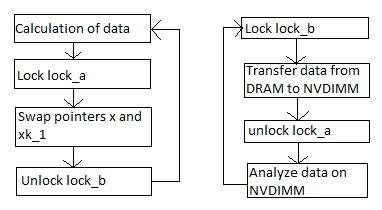
\includegraphics[scale=1]{lock_overview.png}
\caption{A simplified version of how lock works in the program.}
\end{figure}

\subsubsection{Calculation}
The total time for calculation are measured before and after the while-loop. One thread will start the time measurement at line 3 and the measurement will be ended by one thread at line 33.
The calculation starts with a while-loop at line 5. It will be repeated 5000 times. There is a barrier at line 6 that will synchronize all the threads. One thread will enter a single bracket a line 7 and increase the variable n by one, zero out the variables diff and Wk\_1 and calculate one part of the calculation that only need to be done by one thread at line 11.

The calculation of data will happens at line 17. All threads will enter the for-loop at line 18, this for-loop will pass through all the nodes in the array. A temporary variable is created at line 20, this is to ensure that data is only stored at the end of the for-loop. Each thread will then enter a second for-loop at line 21. The arrays that begins with CRS is part of a compressed sparse matrix, that means that a 2D-array has been turned into a 1D-array in order to perform faster. The for-loop will add together edges that is connected to node i, they will be stored in the double\_temp variable. Once out of the array the double\_temp will be multiplied with a constant d at line 25 and added together with the Wk\_product at line 27, this is a variable that was calculated by one thread in line 13.
The double\_temp value will be written to array at line 28.

One thead will enter the single bracket at line 36 and will start a new time measurement at line 38. This time measurement will measure how much time the calculation threads must wait for the analyze threads to finish. Once the analyze threads have unlocked lock\_a the thread will pass through the lock and lock it again at line 39. It will also end the time measurement at line 40 and add the time waited to the iteration\_idle\_time variable. This variable represent the total amount of time the calculation threads have been idle.
At line 42-44 the arrays x and xk\_1 will be swapped. At line 46 the thread will unlock the lock\_b, this will allow the analyze threads to do their jobs. The threads will then return to the beginning of the while-loop at line 5 and repeat the process if n is lower than 5000.


\begin{lstlisting}[caption=Calculation]
#pragma omp single
{
	iteration_time = mysecond();
}
while( n<5000 ){ 
	#pragma omp barrier
	#pragma omp single
	{
		n++;
		diff=0.0;	
		Wk_1=0;
		//completes the first part of the formula.
		Wk_1_product = (omd + (d*Wk_1))*iN;
	}
	
	/* Calculation of Data */
	#pragma omp for reduction(max:diff)
	for( i=0; i<nodes; i++){
		//This is A*x^k-1
		double_temp = 0;
		for( j=CRS_row_ptr[i]; j<CRS_row_ptr[i+1]; j++){ 
			double_temp += CRS_values[j] * xk_1[CRS_col_idx[j]];
		}
		//d*Ax^k-1
		double_temp *= d;
		//Adding the first part and second part together.
		double_temp += Wk_1_product;
		x[i] = double_temp;

		//Comuting the difference between x^k and x^k-1
		//and adds the biggest diff to diffX[thread_id]
		if( x[i]-xk_1[i] > diff )
			diff = x[i] - xk_1[i];
	}

	#pragma omp single
	{
		temp_time = mysecond();
		omp_set_lock(&lock_a);
		iteration_idle_time += mysecond() - temp_time;

		temp_x = xk_1;
		xk_1 = x;
		x = temp_x;
		
		omp_unset_lock(&lock_b);
	}
}//end of while-loop
#pragma omp single
{
	iteration_time = mysecond() - iteration_time;
}
\end{lstlisting}
\subsubsection{Analyze}
The time will be measured before and after the while-loop that start at line 1. The if test for this while-loop has been moved to the end of the while-loop, that is why the it test at line 1 is 1==1 and will allways be true. 
One thread will enter the single bracket at line 2 and start a time measurement that will measure the idle time of the analyze threads. The threads will wait until the calculation threads unlocks the lock\_b. When its unlocked the thread will pass through line 5 and lock lock\_b again. It will also add the time waited to the variable transfer\_idle\_time. The thread will then start a new time measurement at line 7, this measurement will measure the time it takes to transfer data from DRAM to NVDIMM. the variable average will be turned to zero at line 8.
At line 11-14 all the threads will work together to transfer the xk\_1 array from DRAM to NVDIMM.
Once done one thread will enter a new single at line 15. The thread will then end the time measurement at line 17 and add the time taken to transfer the data to the variable DRAM\_to\_NVM\_time.
It will then unlock lock\_a at line 18, this will allow the calculation threads to swap x and xk\_1. The thread will also start a new time measurement at line 19, this measurement will measure how long it takes for the threads to analyze the data. From line 22-25 is where the data gets analyzed, in this case its just an average of all the data. 
The threads will synchronize at a barrier at line 26. One thread will enter the single thread at line 27 and will divide the sum of all the nodes with the number of nodes.
It will then end the time measurement at line 30 and add it to the total time it takes to analyze the data.
All the threads will then go through an if test at line 33. This test will always be true until the calculation threads changes the iteration\_ongoing variable from 1 to 0.This will only be done when calculation threads are done with calculation and left their while-loop that was explained above.

\begin{lstlisting}[caption=Analyze]
while(1==1){
	#pragma omp single
	{
		temp_time = mysecond();
		omp_set_lock(&lock_b);
		transfer_idle_time += mysecond() - temp_time;
		temp_time = mysecond();
		average=0.0;
	}
	/* Transfer of array from DRAM to NVDIMM */
	#pragma omp for
	for(i=0; i<nodes; i++){ 
		D_RW(nvm_values)[i]=xk_1[i];
	}
	#pragma omp single 
	{
		DRAM_to_NVM_time += mysecond() - temp_time;
		omp_unset_lock(&lock_a);
		temp_time = mysecond();
	}
	/* Analyzations of data */
	#pragma omp for reduction(+ : average)
	for(i=0;i<nodes;i++){
		average += D_RO(nvm_values)[i];
	}
	#pragma omp barrier
	#pragma omp single
	{
		average /= nodes;
		Analyse_time += mysecond() - temp_time;
	}
	//if sentence for exiting while-loop.
	if(iteration_ongoing==0){
		break;
	}
}
\end{lstlisting}

\subsubsection{Prediction}
Table \ref{tab:nvmPredictions} shows the time prediction that the code above will take. Column one and two shows the number of DRAM and NVDIMM threads that are being used. The last three columns shows the predicted times for data generation on DRAM, transfer of data from DRAM to NVDIMM and the analyzing of data in NVDIMM. The speeds used to predict times comes from benchmarks in section \ref{section:NVM-NVM} and \ref{section:DRAM-NVM}. The calculation of the data traffic data generation and analyzing of data in this prediction is the same as the one in figure \ref{fig:DramOnlyMath1} and \ref{fig:DramOnlyMath2}. The data traffic for the data transfer from DRAM to NVDIMM is calculated in figure \ref{fig:DramOnlyMath3}.
\begin{figure}
\[
	\frac{nodes*5000*8}{1000000}
\]
\caption{Calculation of data traffic generated by transferring data from DRAM to NVDIMM, result is measured in megabytes.}
\label{fig:DramOnlyMath3}
\end{figure}
\begin{table}[!hbtp]
\begin{tabular}{ |c|c|c|c|c| } 
\hline
DRAMTheads & NVMthread & DataGen & transfer & analyze \\
\hline
15 & 1 & 151.98 & 178.70 & 1053.27 \\
\hline
14 & 2 & 160.61 & 87.38 & 530.92 \\
\hline
13 & 3 & 172.54 & 58.43 & 346.94 \\
\hline
12 & 4 & 180.99 & 42.47 & 253.36 \\
\hline
11 & 5 & 194.20 & 34.18 & 210.49 \\
\hline
10 & 6 & 211.95 & 28.30 & 170.48 \\
\hline
9 & 7 & 233.21 & 24.10 & 144.89 \\
\hline
8 & 8 & 255.74 & 20.93 & 127.65 \\
\hline
7 & 9 & 291.06 & 18.83 & 112.20 \\
\hline
6 & 10 & 323.34 & 16.76 & 103.76 \\
\hline
5 & 11 & 377.42 & 15.14 & 94.14 \\
\hline
4 & 12 & 451.44 & 13.94 & 84.20 \\
\hline
3 & 13 & 584.30 & 12.97 & 79.98 \\
\hline
2 & 14 & 842.55 & 12.00 & 72.87 \\
\hline
1 & 15 & 1563.66 & 11.16 & 69.04 \\
\hline
\end{tabular}
\caption{Time prediction in seconds, Data generation, data transfer and analyzing of data.}
\label{tab:nvmPredictions}
\end{table}

\subsubsection{Result}
\begin{table}[!hbtp]
\begin{tabular}{ |c|c|c|c|c|c| } 
\hline
Total & DataGen & Analyze & DataGen & DataGen & Total \\
\hline
threads & Threads & threads & time & idle time & Time \\
\hline
16 & 15 & 1 & 102.35 & 849.87 & 952.37 \\
\hline
16 & 14 & 2 & 105.89 & 402.37 & 508.35 \\
\hline
16 & 13 & 3 & 112.69 & 274.05 & 386.80 \\
\hline
16 & 12 & 4 & 117.66 & 181.92 & 299.63 \\
\hline
16 & 11 & 5 & 123.18 & 126.36 & 249.58 \\
\hline
16 & 10 & 6 & 130.29 & 90.92 & 221.25 \\
\hline
16 & 9 & 7 & 136.33 & 51.77 & 188.13 \\
\hline
16 & 8 & 8 & 147.03 & 18.63 & 165.69 \\
\hline
16 & 7 & 9 & 169.39 & 3.78 & 173.20 \\
\hline
16 & 6 & 10 & 182.96 & 0.02 & 183.01 \\
\hline
16 & 5 & 11 & 206.64 & 0.00 & 206.67 \\
\hline
16 & 4 & 12 & 246.10 & 0.31 & 246.46 \\
\hline
16 & 3 & 13 & 303.90 & 0.00 & 303.93 \\
\hline
16 & 2 & 14 & 430.30 & 0.00 & 430.34 \\
\hline
16 & 1 & 15 & 804.03 & 0.00 & 804.08 \\
\hline
\end{tabular}
\caption{Result of generating data.}
\label{tab:nvmDataGenerationTimes}
\end{table}

Table \ref{tab:nvmDataGenerationTimes} and \ref{tab:nvmanalyzetimes} are from the same test, they have been split up so they can fit within a page.
Just like in section \ref{section:DramOnlyPrediction} the predictions were not spot on. 
The prediction of data generation and the analyze time in table \ref{tab:nvmPredictions} is always slower than the measured result in table \ref{tab:nvmDataGenerationTimes}. They could serve as a prediction of maximum time needed for the data generation and analyzing of data to complete their tasks. The prediction of the data transfer is less reliable then the others. This is because it predict more time then what the actual time is in the beginning and at the end it predict less time then what is actually needed. It cant be used to predict a maximum time or a minimum time needed for the transfer of data between DRAM and NVDIMM.

The fastest combination of DRAM and NVDIMM thread in this test is when both DRAM and NVDIMM have eight threads. This is also the combination where the combined idle time of the two groups of threads are the lowest which is also the reason why it was the fastest one. 

The fastest combination result in this section is 25 second slower when compared to the fastest result of DRAM only version of the code in table \ref{tab:DramOnlyResult}. It was expected that the NVDIMM version of the code would be slower then the DRAM only version of the code. But still it is possible to assign the DRAM with one set of tasks while the NVDIMM version of the code are doing another set of tasks. The only downside is that it will take longer time. When comparing the extra time a project will take with the lower cost of NVDIMM it might be a compromise someone are willing to make. The challenge might lie in deciding how many threads to assigned to the NVDIMM because the prediction I tried to make was not very accurate.

\begin{table}[!hbtp]
\begin{tabular}{ |c|c|c|c|c|c|c| } 
\hline
Total & DataGen & Analyze & Transfer & DRAM-NVM & Analyze & Total \\
\hline
threads & Threads & threads & idle time & time & time & Time \\
\hline
16 & 15 & 1 & 0.03 & 166.02 & 786.30 & 952.37 \\
\hline
16 & 14 & 2 & 0.04 & 84.74 & 423.54 & 508.35 \\
\hline
16 & 13 & 3 & 0.03 & 70.52 & 316.22 & 386.80 \\
\hline
16 & 12 & 4 & 0.01 & 51.48 & 248.09 & 299.63 \\
\hline
16 & 11 & 5 & 0.03 & 43.15 & 206.36 & 249.58 \\
\hline
16 & 10 & 6 & 0.03 & 44.56 & 176.63 & 221.25 \\
\hline
16 & 9 & 7 & 0.10 & 34.79 & 153.22 & 188.13 \\
\hline
16 & 8 & 8 & 0.03 & 31.22 & 134.42 & 165.69 \\
\hline
16 & 7 & 9 & 16.01 & 36.38 & 120.80 & 173.20 \\
\hline
16 & 6 & 10 & 51.34 & 28.85 & 102.81 & 183.01 \\
\hline
16 & 5 & 11 & 90.16 & 26.39 & 90.11 & 206.67 \\
\hline
16 & 4 & 12 & 127.23 & 28.67 & 90.41 & 246.46 \\
\hline
16 & 3 & 13 & 205.38 & 22.83 & 75.71 & 303.93 \\
\hline
16 & 2 & 14 & 338.74 & 21.71 & 69.86 & 430.34 \\
\hline
16 & 1 & 15 & 718.38 & 20.60 & 65.07 & 804.08 \\
\hline
\end{tabular}
\caption{Result of transfer data to NVDIMM and analyzing the data.}
\label{tab:nvmanalyzetimes}
\end{table}



%%%%%%%%%%%%%%%%%%%%%%%%%%%%%%%%%%%%%%%%%%%%%%%%%%%%%%%%%%%%%%
%
%%%%%%%%%%%%%%%%%%%%%%%%%%%%%%%%%%%%%%%%%%%%%%%%%%%%%%%%%%%%%%

\begin{comment}
\begin{table}[!hbtp]
\begin{tabular}{ |c|c|c|c|c|c|c|c|c| } 
\hline
 Total & DataGen & Analyze & DataGen & DataGen & Transfer & DRAM\-NVM & Analyze & Total \\
\hline
 threads & Threads & threads & time & idle time & idle time & time & time & Time \\
\hline
16 & 15 & 1 & 102.35 & 849.87 & 0.03 & 166.02 & 786.30 & 952.37 \\
\hline
16 & 14 & 2 & 105.89 & 402.37 & 0.04 & 84.74 & 423.54 & 508.35 \\
\hline
16 & 13 & 3 & 112.69 & 274.05 & 0.03 & 70.52 & 316.22 & 386.80 \\
\hline
16 & 12 & 4 & 117.66 & 181.92 & 0.01 & 51.48 & 248.09 & 299.63 \\
\hline
16 & 11 & 5 & 123.18 & 126.36 & 0.03 & 43.15 & 206.36 & 249.58 \\
\hline
16 & 10 & 6 & 130.29 & 90.92 & 0.03 & 44.56 & 176.63 & 221.25 \\
\hline
16 & 9 & 7 & 136.33 & 51.77 & 0.10 & 34.79 & 153.22 & 188.13 \\
\hline
16 & 8 & 8 & 147.03 & 18.63 & 0.03 & 31.22 & 134.42 & 165.69 \\
\hline
16 & 7 & 9 & 169.39 & 3.78 & 16.01 & 36.38 & 120.80 & 173.20 \\
\hline
16 & 6 & 10 & 182.96 & 0.02 & 51.34 & 28.85 & 102.81 & 183.01 \\
\hline
16 & 5 & 11 & 206.64 & 0.00 & 90.16 & 26.39 & 90.11 & 206.67 \\
\hline
16 & 4 & 12 & 246.10 & 0.31 & 127.23 & 28.67 & 90.41 & 246.46 \\
\hline
16 & 3 & 13 & 303.90 & 0.00 & 205.38 & 22.83 & 75.71 & 303.93 \\
\hline
16 & 2 & 14 & 430.30 & 0.00 & 338.74 & 21.71 & 69.86 & 430.34 \\
\hline
16 & 1 & 15 & 804.03 & 0.00 & 718.38 & 20.60 & 65.07 & 804.08 \\
\hline
\end{tabular}
\end{table}
\end{comment}

\begin{comment}
\begin{table}[!hbtp]
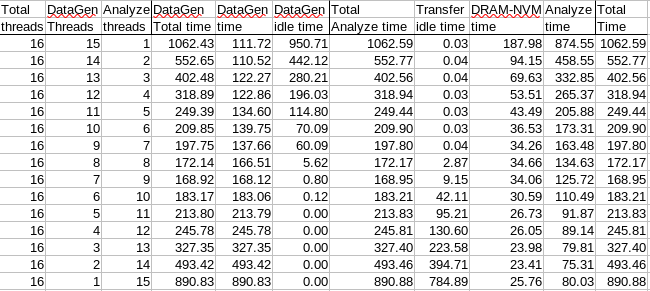
\includegraphics[scale=0.7]{Simulation/Simulation_time.png}
\caption{Simulation with both NVDIMM and DRAM}
\end{table}

\begin{table}[!hbtp]
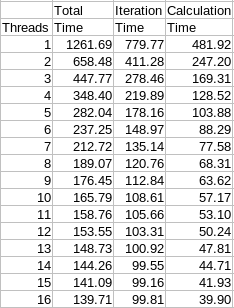
\includegraphics[scale=0.7]{Simulation/DRAM_only.png}
\caption{Simulation with only DRAM, n=16M}
\end{table}
\begin{table}[!hbtp]
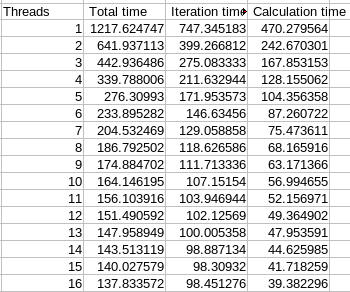
\includegraphics[scale=0.7]{DRAM_only_16M.png}
\caption{Simulation with only DRAM, n=16M}
\end{table}
The generation of data happens inside a while-loop that will repeat the generation and analyzing of data 5000 times. The total time is measured by taking the time before and after the while-loop. The analyzing time is measured the same way by taking the time before and after the analyzing part of the program. Data generation time is measured by subtracting the analyze time from the total time. All the time measurements are made inside a pragma omp single so there are no reason to be worried if the mysecond-method is thead-safe. The mysecond-method have been copied from the original stream benchmark.
All the arrays used in the code have been subjected to first touch before the time is measured.
\end{comment}

\begin{comment}
\begin{table}[!hbtp]
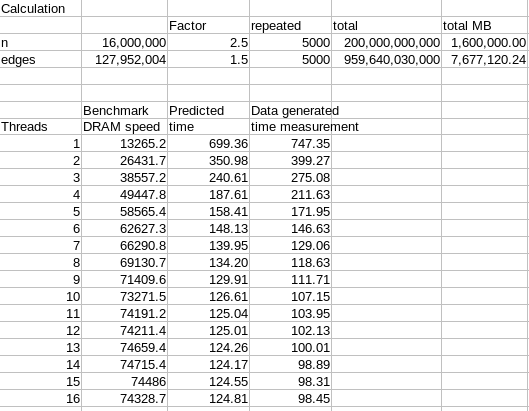
\includegraphics[scale=0.7]{DRAM_only_DataGeneration_16M.png}
\caption{Prediction of time taken for data generation, n=16M}
\end{table}
\end{comment}


\begin{comment}
\begin{table}[!hbtp]
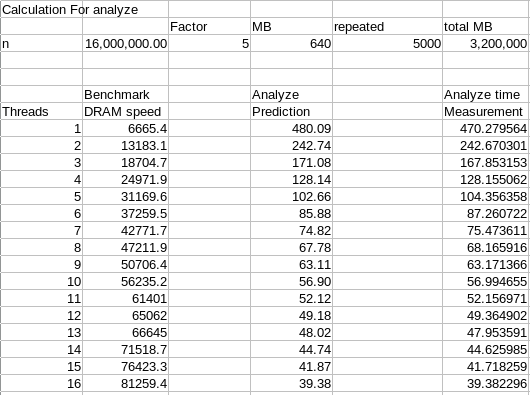
\includegraphics[scale=0.7]{DRAM_only_Analyze_16M.png}
\caption{Prediction of time taken for analyzing the data, n=16M}
\end{table}
\end{comment}

\begin{comment}
\clearpage
\subsubsection{Stream benchmark, sum}
This benchmark is the STREAM benchmark with an added benchmark. The sum is found by adding all the elements into a single variable. The STREAM benchmark was changed by increasing several array from four to five and added the sum benchmark after the four other benchmark. 
The STREAM benchmark for NVDIMM is the same as the one described above, but the code has been changed so the benchmark will read and write to the NVDIMM.

\begin{table}[!hbtp]
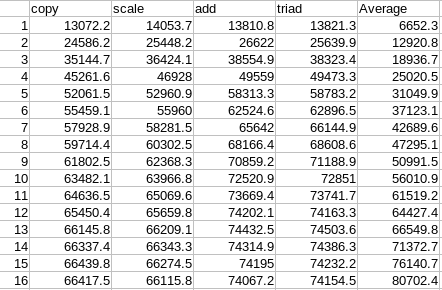
\includegraphics[scale=0.7]{Stream_benchmark.png}
\caption{New Stream benchmark, DRAM}
\end{table}

\begin{table}[!hbtp]
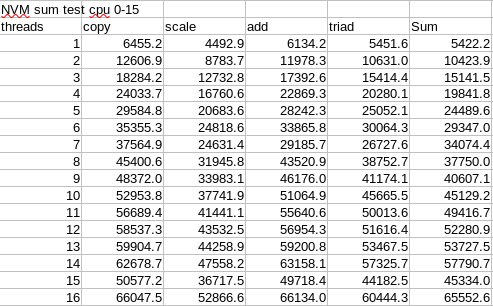
\includegraphics[scale=0.7]{Stream_NVM_sum.png}
\caption{New Stream benchmark, NVM}
\end{table}
\end{comment}

\begin{comment}
\clearpage
\subsubsection{Calculation only} 
\begin{table}[!hbtp]
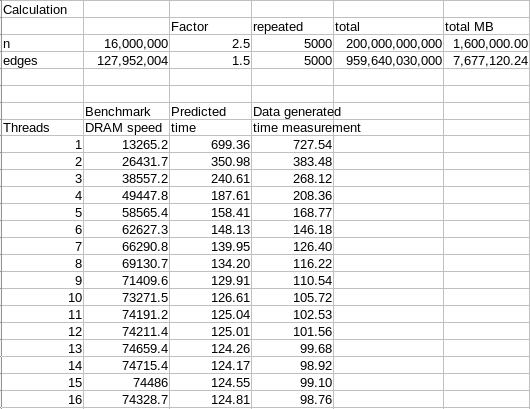
\includegraphics[scale=0.7]{Benchmark_only_prediction.png}
\caption{Prediction of time taken for calculation of the data, with a code that only do calculation}
\end{table}
\end{comment}

\begin{comment}
\clearpage
\subsection{NVDIMM Analyze only}
\begin{table}[!hbtp]
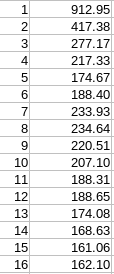
\includegraphics[scale=0.7]{NVDIMM_analyze_only}
\caption{Mearsurement of analyzations only on NVDIMM.}
\end{table}
\end{comment}


\begin{comment}
\clearpage
\subsubsection{Old}
\begin{table}[!hbtp]
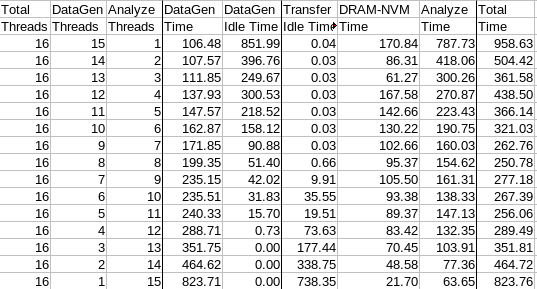
\includegraphics[scale=0.7]{Simulation_NVM_2.png}
\caption{Simulation with both NVDIMM and DRAM}
\end{table}

getconf LEVEL1\_DCACHE\_LINESIZE have been used to find the cacheline size in bytes.

\begin{table}[!hbtp]
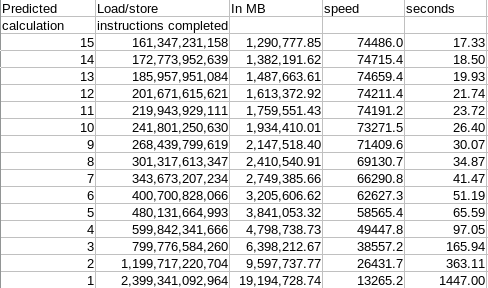
\includegraphics[scale=0.7]{Predicted_calculation.png}
\caption{Predicted calculationbased on papi.}
\end{table}

\begin{table}[!hbtp]
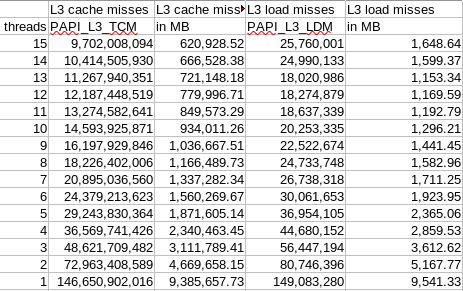
\includegraphics[scale=0.7]{Predicted_calculation_3.png}
\caption{Tried to split load and store misses. Server do not support store misses.}
\end{table}

\begin{table}[!hbtp]
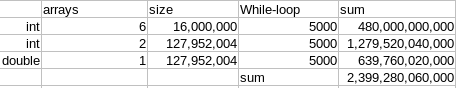
\includegraphics[scale=0.7]{Array-counting.png}
\caption{Manually counted the number of int and double tranfers.}
\end{table}

\begin{table}[!hbtp]
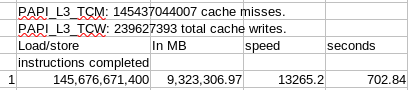
\includegraphics[scale=0.7]{Predicted_calculation_2.png}
\caption{Predicted calculationbased on papi with L3.}
\end{table}

\begin{table}[!hbtp]
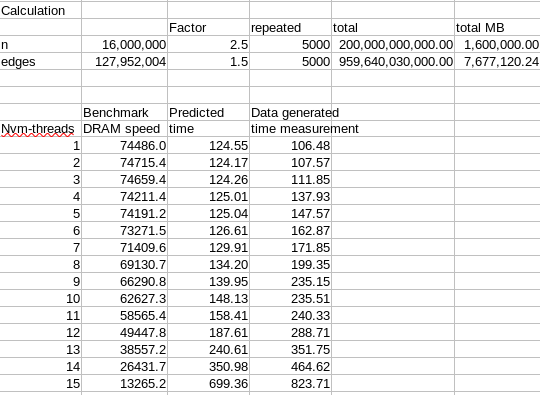
\includegraphics[scale=0.7]{Datagen_prediction_NVM.png}
\caption{Time prediction, data generation}
\end{table}

\begin{table}[!hbtp]
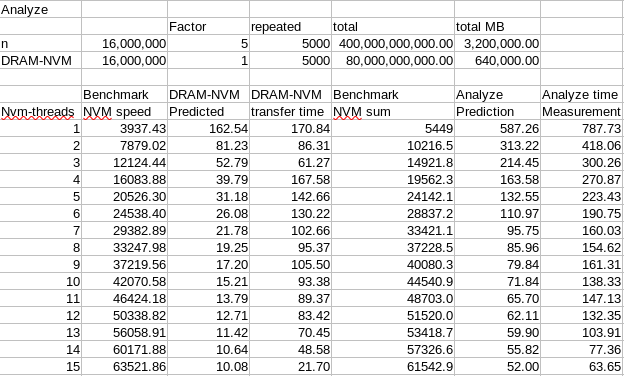
\includegraphics[scale=0.7]{Analyze_prediction_NVM.png}
\caption{Time prediction, transfer and analyze}
\end{table}

\clearpage
\subsection{2D-array test}
\begin{lstlisting}[caption=Kildekode]
https://github.com/SveinGunnar/Master_Thesis_2020/tree/master/ArrayCopyTest
\end{lstlisting}
\begin{table}[!hbtp]
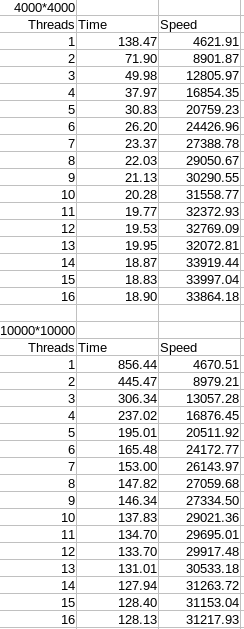
\includegraphics[scale=0.7]{2D_array_test.png}
\caption{2D-Array test}
\end{table}
\end{comment}

\end{document}
